\chapter{Introduction} \label{chap:intro}

\section{Problem}
\begin{itemize}
\item location-based applications broad appeal (navigation, robotics, gaming, asset tracking, ...)
\item no GPS, loss of signal, or very bad accuracy
\end{itemize}

\section{Idea}

Use approach from robotics.

Ein Grund Q/A [Apple intro], says it is not possible to show precise location.

UseCase:
\begin{itemize}
  \item (assets management, staff tracking,) indoor tourist guiding in museums, train stations, airport, shopping complex \citep{wang:bt_pos}
  \item example ADAMANT (airport travelers guide) \citep{wang:bt_pos}
\end{itemize}

Requirements:
\begin{itemize}
\item low cost
\item public available device
\item cross platform
\item every thing on device \citep{wang:bt_pos}
\item easy-to-deploy \citep{wang:bt_pos}
\end{itemize}

Map with beacon positions

\section{Structure}
\textit{Explain the documents structure}


\chapter{Fundamentals}\label{chap:fundamentals}

In this chapter, we first introduce the fundamentals of localization. Afterwards, we give an overview of different localization algorithms being used in related work. Then, we point out the reasons for choosing the particle filter for this project, to finally introduce the algorithm itself.

\section{Fundamentals of Localization}

Localization, aka.\ positioning, is the process of estimating the position of an object in its environment. Usually, the object's environment is being defined as a coordinate system. One of the most popular coordinate systems is the \emph{World Geodetic System 19984 (WGS84)}, which describes a position globally on earth in longitude and latitude. Sometimes, it is sufficient to use a local coordinate system; for instance, a two or three dimensional cartesian coordinate system. Indoor localization is one example, where it is sufficient to use a local coordinate system, because the object's position is limited to a defined map, resp.\ the scope of the building.

\paragraph{Location Types}
Locations can be of four types. A \emph{physical location} is described in coordinates on a map. \emph{Symbolic locations} such as ``in the living room'' or ``on the small table in the kitchen'', are often used by humans. If all objects are sharing a frame of reference, like chess pieces on a chess board, the type of location is called a \emph{absolute location}. If an object has its own reference frame as for instance, ``I am two meters away from the door'', which often includes a proximity value, it is called a \emph{relative location} \citep{IEEE:survey_wireless_indoor_pos}.

\paragraph{System Topology}
Usually, a pure wireless localization system consists of at least one transmitter that emits some sort of signal, and one or more receivers, respectively a measuring units. The system's topology can be \emph{remote positioning}, which means that the transmitters position is being estimated by using the measurements of multiple measuring units that are deployed at fixed locations. The position estimation takes place in a separate component which uses the measurements as input. If the measurement unit is mobile and estimates its own position, by collecting the signals of fixed transmitters, the system's topology is called \emph{self-positioning}. \emph{Indirect remote positioning} is basically the same as self-positioning, but the collected measurements are send via some data connection to an external service, which does the position estimation. If the system's topology is basically remote positioning, but the measurements are transferred via a wireless data link to the mobile side, the topology is called \emph{indirect self-positioning} \citep{IEEE:survey_wireless_indoor_pos}.

Besides a pure wireless localization systems, which just use wireless signals for the positioning, also other systems, often used in the area of mobile robotics, do exist. Robots are often equipped with sensors, such as laser scanners or ultrasonic sensors, to measure distances to obstacles. Wheel and chain based robots are usually also equipped with odometers, others do have accelerometers and rotation rate sensors to estimate the traveled distance. The used localization algorithms are able to combine different sensors to provide a more accurate estimation \citep{thrun:prob_robo}. Mobile robots, especially if they operate autonomous, are usually self-positioning, or indirect remote positioning systems, which often depends on their system's hardware capabilities. Remote positioning as well as indirect self-positioning systems are rarely the case in the field of mobile robots.

\paragraph{Uncertainty}
To be able to estimate an accurate position, localization systems need to be able to accommodate uncertainty. According to \citet{thrun:prob_robo}, uncertainty in robotic systems has several reasons.

One reason is its \emph{environment}. If a robot works together with humans, the environment is very dynamic and unpredictable, because the robot does not know for instance, where a human moves next. Of course, robots are equipped with \emph{sensors} to recognize obstacles like humans, but sensors do also cause uncertainty. On one side, they are limited, e.g.\ a camera has a specific resolution, and on the other side, noise unpredictably influences their measurements. Typically, robots do have \emph{actuators}, for instance motors to move in its environment. Actuators are limited in their precision. Additionally, their successive physical components, for instance a robots wheels on a varying surface, may cause unpredictable effects. To allow robots to operate in a physical environment, models of it are being used. \emph{Models} are abstractions, which approximate a certain object or behavior.  Thus, information is being lost, and additionally every model has some inaccuracy. Robotic systems work in a real-time environments. Due to computational reasons, their \emph{algorithms} cannot really operate in real-time. In reality, a physical property changes continuously, but a robot's measurements can just being processed in certain time steps, which causes inaccuracy. 

All mentioned factors together do cause large uncertainty. Thus, the system needs to be able to accommodate it.

\paragraph{Localization Problems}
Localization is not always the same. There are different localization problems depending on the environment and use-case of the application. According to \citet{thrun:prob_robo} the following problems do exist:
\begin{itemize}
	\item \textbf{Local vs.\ Global Localization} If the (robot's) initial pose is known when the localization begins to start and thus just a so called position tracking is necessary to know after a certain time what the new position is, it is called \emph{local localization}. If the initial pose is unknown, thus the robot's position can by anywhere on the map, it is called \emph{global localization}. These types of algorithms are more difficult than position tracking. Global localization solves also the \emph{kidnapped robot} problem, which means that a robot is being placed on a different position during the position estimation. Of course, that is not very typically, but by solving this problem the robot is also able to recover if the algorithm is stuck in a state where it never will find out its real position.
	\item \textbf{Static vs.\ Dynamic Environments} In a \emph{static environment} the robot, resp.\ the localizing object, is the only object that changes its position over time. All obstacles and other objects keep their position forever. In a \emph{dynamic environment} other objects besides the localizing object can also change their pose. Typical objects in a dynamic environment are humans, furnitures like chairs or doors that sometimes are being closed or not fully opened.
	\item  \textbf{Passive vs.\ Active Approaches} If the localization algorithm is able to control a robots motion it is an \textbf{active approach}. By influencing the robot's motion the algorithm can move the robot if the localization is stuck and needs more information from maybe another point of view of a room to decide what its position is. \textbf{Passive} algorithms just observe the robot's motion but cannot influence it. Usually, active approaches are build upon passive ones.
	\item \textbf{Single-Robot vs.\ Multi-Robot} \textbf{Single-Robot} localization means, that the robot just needs to localize itself. \textbf{Multi-Robot} localization requires of course multiple robots in the same area. It builds up on single-robot localization, thus each robot can estimate its position be itself. It brings up new opportunities if the robots can see each other and are able to communicate to exchange their estimated poses.
\end{itemize}

\paragraph{Performance Metrics}
To be able to compare different localization systems and algorithms, we introduce the following criteria, which are being recommended by \citet{IEEE:survey_wireless_indoor_pos}, because also from our point of view the system's accuracy is not sufficient enough for evaluation purposes.
\begin{itemize}
	\item \textbf{Accuracy} is the error in the estimated position. It is the Euclidean distance between the estimated and the real position.
	\item \textbf{Precision} takes also the consistency into account. Liu et al defines it as the result of ``the cumulative probability function[s] (CDF) of the distance error'', for instance 90~\% location precision within 2~meters ($CDF(2m) = 0.9$).
	\item \textbf{Complexity} may depends on several factors, the required hardware, the software complexity, the algorithms complexity, the necessary infrastructure, etc. Liu et al are just focussing on software resp. computing complexity.
	\item \textbf{Robustness} expresses, if a system can deal with wrong sensor data, unexpected values or even no sensor data in a time interval.
	\item \textbf{Scalability} ensures, that a system can be extended or reduced in space or in density of the transmitters or measurement units.
	\item \textbf{Cost} depends on several factors. The financial cost is a very important factor. It depends on the hardware, implementation and installation costs. The energy consumption, which in the end also reflects in financial cost, is also an important factor. The factor time should also not negligible. The amount of time it takes to deploy and maintain such a system can be enormous.
\end{itemize}


\section{Localization Algorithms \& Related Work}

\subsection{Triangulation}
Triangulation is a well-studied localization method which relies on triangle's geometric properties \citep{IEEE:survey_wireless_indoor_pos, wang:bt_pos}. Triangulation is the hypernym of the two characteristics \emph{lateration} and \emph{angulation}.

\begin{figure}[width=0.9\textwidth, height=0.4\textheight]
\subfloat[Lateration]{
  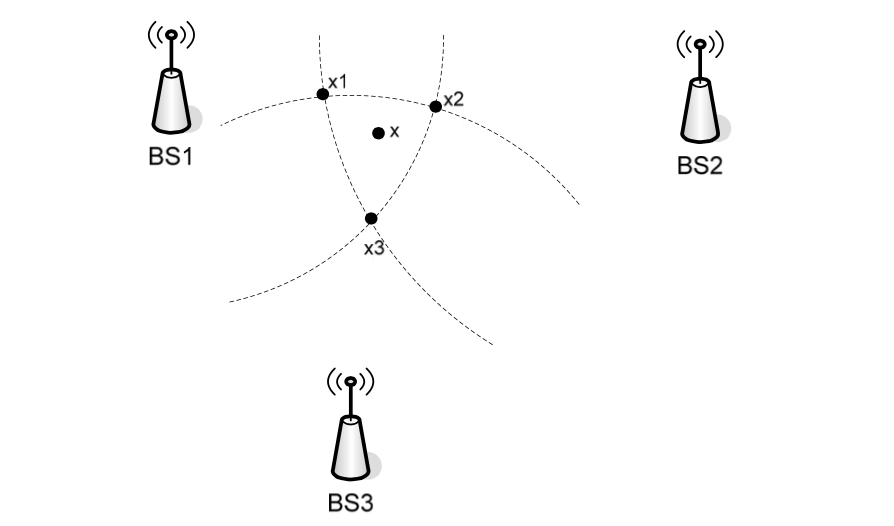
\includegraphics[width=0.45\textwidth]{figures/lateration}
  \label{fig:lateration}
}
\subfloat[Angulation]{
  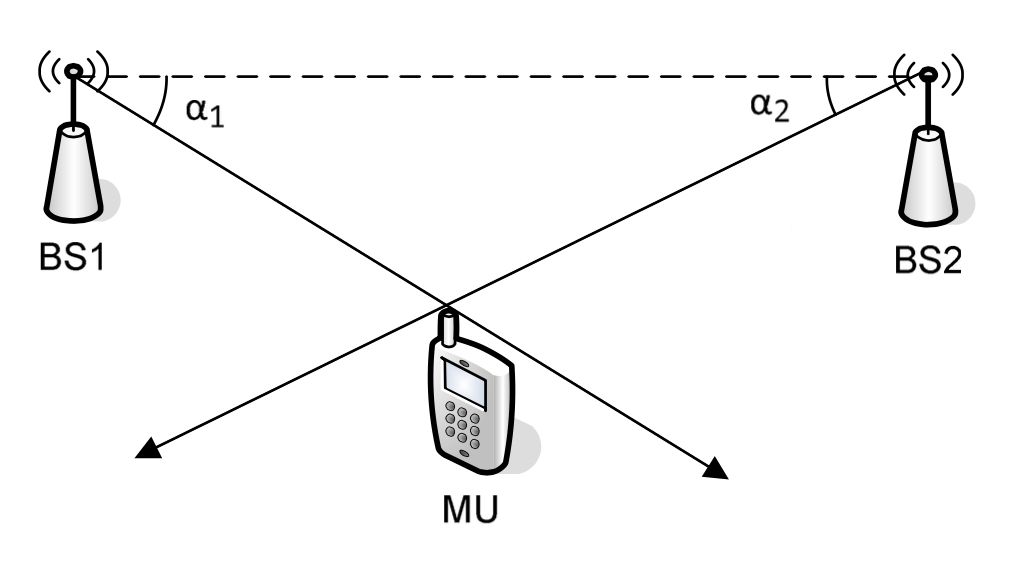
\includegraphics[width=0.45\textwidth]{figures/angulation}
  \label{fig:angulation}
}
\caption {Triangulation methods. Source:~\citep{wang:bt_pos}}
\label{fig:triangulation}
\end{figure}

Lateration estimates the location based on the distances from the measuring unit to the transmitters. To precisely estimate a position, three base stations are required. The measuring unit measures the distance to each basestation and puts a circle with the radius of the measured distance around the basestation. The circles's common intersection point, is the exact position of the mobile unit. In 2D space at least three signals must be received, in 3D four signals are required. According to \citet{wang:bt_pos}, one common intersection point exists just in theory. In practice errors, due to obstacles and imperfect propagation models, do influence the distances. Thus, no common intersection point exists. Figure~\ref{fig:lateration} depicts the case. Nevertheless it is possible to estimate the mobile units position by using methods such as least-square, three-boarder, or the centroid-method \citep{wang:bt_pos, IEEE:survey_wireless_indoor_pos}.  
The distance for lateration can be estimated with different methods. According to \citet{IEEE:survey_wireless_indoor_pos}, the distance between the measuring unit and the transmitter is directly proportional to the signal's propagation time.
\emph{\ac{TOA}} uses this fact to estimate the distance by measuring the signals travel time. Therefor, the transmitted signal contains the timestamp of its transmission. Thus, the clocks of all transmitters and measuring units, that are participating at the system need to be precisely synchronized in order to do a correct estimation, which is a not trivial problem. According to \citet{kotanen:exp_local_pos_bt}, a timing difference of  $1.0~\mu s$ causes an error of 300~m in distance.
To overcome this disadvantage, a similar method called \emph{\ac{RTOF}} can be used. This method requires all components to be able to receive and transmit signals. The transmitter sends the signal, it is being received and immediately being returned by the mobile unit. Thus the transmitter sets the timestamp and compares it with its current timestamp when the signal arrives. A relative time synchronization is sufficient enough. But \acs{RTOF} has another problem. The signal is being delayed by the processing time, the unit requires to receive and to send back the signal to the original source.
The \emph{\ac{TDOA}} method calculates the distance from the different arrival times at the measuring units. Therefor, the measuring units need to be connected with each other to exchange the timestamps of the signals's arrival and to precisely synchronize their timestamps. The clocks's differences should not exceed tens of nanoseconds \citep{kotanen:exp_local_pos_bt}. The mobile unit, resp.\ the transmitter, does not need to be synchronized. 
All of the above mentioned methods are based on times and thus need precisely, synchronized or relatively synchronized clocks. According to \citet{IEEE:survey_wireless_indoor_pos}, \acs{TOA} and \acs{TDOA} require a \acs{LOS} channel between transmitter and measuring unit in an indoor environment, because time and angle of the signals arrival is being affected by the multipath effect, which is a problem of radio propagation. Wireless technologies, such as Bluetooth and WiFi do have a \emph{\ac{RSSI}} property, which expresses indirectly the signal's RX power level, measured by the bluetooth device \citep{kotanen:exp_local_pos_bt}. As a consequence, instead of measuring times to calculate the distance between sender and receiver, the loss of the signal strength on its path between the two units can be measured. Therefor, the measuring unit needs to know the origin \ac{RSS} of the emitted signal. As mentioned by \citet{IEEE:survey_wireless_indoor_pos}, different theoretical and empirical models can be used to translate the signals attenuation to a distance estimation, but also these models do not always hold due to multipath fading and shadowing in indoor environment.

Instead of using distances for the positioning, angulation uses the angles to multiple measurement units, as shown in figure~\ref{fig:angulation}. In 2D space two angles, in 3D space three angles are sufficient for the positioning. But, to measure the angle of an arriving signal, special, directional antennas or arrays of antennas are required. In the \emph{\ac{AOA}} method, the intersection point of the straights with the measured angles is the mobile units position. Therefor, highly precise angles need to be measured, which is a big problem in wireless environments doe to multipath reflections and shadowing, as already mentioned before \citep{IEEE:survey_wireless_indoor_pos, wang:bt_pos}.

\citet{wang:bt_pos} are using Bluetooth to implement a indoor positioning system for mobile devices like smartphones. The system is based on triangulation methods, resp.\ on lateration using \acs{RSS} for the distance estimation. During their research, they evaluated the least-square, three-border, and centroid method for the position estimation. They found out, without mentioning any details, that all three methods deliver satisfying results, if the mobile unit receives accurate \acs{RSSI} readings and a proper path loss model is being used to calculate the distances. The also analyzed the effect of a human body on the line between transmitter and measuring unit, and found out, that the signal is weakened by 6 --- 8 dB, which results in a few meters due to the fact that dB is a logarithmic unit. To improve the estimation accuracy, they propose to filter the \acs{RSSI} readings by a average or weighted filter, because the \acs{RSSI} values are fluctuating due to fading effects.

\citet{oksar:bluetooth} also uses Bluetooth, based on \acs{RSSI} readings, for their indoor localization. But, compared to \citet{wang:bt_pos}, this time the mobile units are the transmitters, and the measuring units are the fixed base stations with known position, thus its system topology is remote positioning. They defined a root-mean-square-error function, which compares ``the ratio of the square of distances to the base stations'' with ``the ratio of the signal levels'' \citep{oksar:bluetooth}. The used distances are being calculated for assumed discrete positions of the transmitter. As shown by \citet{oksar:bluetooth}, the better the assumed position matches the real position, the smaller is the result of the error function. Therefore, they assumed, that the received \acs{RSS} decreases proportional to the squared distance. Thus, compared to \citet{wang:bt_pos}, they are not directly calculating the distance between the transmitter and the measuring unit. In their experiment they came up in the best case with a root-mean-square-error of 2.309 meters of localization accuracy. But they also mention, that in a real live applications the points are most probably non-discrete points, thus some changes are necessary.

\citet{hoflinger:acoustic} developed an acoustic indoor localization system called ASSIST which stands for \emph{Acoustic Self-calibrating System for Indoor Smart phone Tracking}. According to \citet{hoflinger:acoustic}, the system can track a smartphone with an error of 25~cm. The smartphone sends out a high frequency acoustic signal using its speaker, which is not being recognizable for humans. The signal's ``amplitude $A$ of sound decreases with distance $r$ according to $A \sim 1/r$''. To detect the signals, fixed measuring units with a sensitive MEMS microphone are being used. Despite the decreasing amplitude, they can detect the signals in 70\% up to 10~m distance. For the position estimation the system uses the \acs{TDOA} method. Therefor, the measuring units are being connected via a wired network, which is at the same time the units power supply. The network is being used to synchronize the units timestamps and to exchange the measured timestamps. According to \citet{hoflinger:acoustic} also the acoustic signals suffer from echos and reflections caused by multipath propagation. To calculate a robust location, outliers are compensated by using particle and Kalman filter. They also mention, that the system can also use inertial smartphone sensors, such as accelerometer, gyroscope, and magnetometer, besides the acoustic infrastructure \citep{hoflinger:acoustic, hoflinger:assist}.

Further research projects based on triangulation methods are referenced by \citet{IEEE:survey_wireless_indoor_pos}.

\subsection{Scene Analysis} Scene analysis localization algorithms, such as \emph{kNN}, \emph{neural networks}, and \emph{Support Vektor Machine}, are based on machine learning. According to \citet{IEEE:survey_wireless_indoor_pos}, the use of such algorithms requires two stages, the offline and online stage. During the offline stage fingerprints, are bring collected at many positions in the area where the later localization should take place. Most often \acs{RSS} fingerprints are being collected which means, that at a specific position the \acs{RSS} values of all received transmitters are being collected. Then the fingerprints are being stored in a database with their corresponding location. The online phase is the actual runtime phase, where the localization takes place. Therefor, the application also creates a fingerprint of the current received signals. The algorithm then compares the fingerprint, with the fingerprints stored in the database during the offline stage and returns the location of the best matching one. As mentioned by \citet{IEEE:survey_wireless_indoor_pos}, the techniques main challenge is to deal with the signals that are being affected by their environment. The scene analysis's offline stage requires a lot of effort, especially in large environments, which is its major disadvantage. Another disadvantage is, that if the environment changes the \acs{RSS} fingerprints may be change, and thus the offline stage need to be repeated. Our work follows different approaches, thus we are not going into more detail on scene analysis. \citet{IEEE:survey_wireless_indoor_pos} gives a more detailed overview of the above mentioned algorithms.


\subsection{Proximity} The proximity method, which is also known as cell-ID tracking, provides just a relative location information. For the localization, the mobile device listens for signals's of different transmitters. The transmitters's locations are know and can be identified by their identifier. As a result, the mobile device's location is \emph{next to the transmitter's location} with the strongest signal \citep{IEEE:survey_wireless_indoor_pos, wang:bt_pos}. As mentioned by \citet{IEEE:survey_wireless_indoor_pos}, the proximity method is a very simple to implement algorithm. Additionally, it can use different wireless technologies at the same time, such as Bluetooth, WiFi, etc.\, the device needs just to listen for all of them simultaneously. To get a precise position information, lots of transmitters need to be spread over the environment. If there are to less, and their range is up to several meters, the location information is very rough \citep{kotanen:exp_local_pos_bt}. As mentioned before, wireless signal's are heavily influenced by its environment. Consequently, it may also happen that the device location is not optimal due to the fact that the signals are not lowered in the same strength and thus, the device location is being associated with a transmitter that is further away, than another one.

\subsection{Kalman Filter} The \emph{\ac{KF}}, resp. the \emph{\ac{EKF}}, is a technique for filtering and prediction of linear, resp. non-linear, gaussian systems with continuous space, such as a indoor robot localization systems, based on the robot's motion and its measurements. As mentioned before, localization systems should be able to accomodate uncertainty. Gaussian filters express the uncertainty of a state, e.g. a robots position, as the belief in the state. Beliefs are represented as multivariante normal distributions with mean $\mu$ and covariance $\Sigma$.

The algorithm is based on three probabilities. The \emph{state transition probability} $p(x_t | u_t , x_{t-1})$ is the probability for a state $x$ at time $t$ after the transition from state $x$ at time $t-1$ by applying the control $u$ at time $t$. Transferred to the above mentioned robot localization this means, that it expresses the belief in the robot's new position $x_t$ after a certain motion $u_t$ with being at position $x_{t-1}$. The \emph{measurement probability} $p(z_t|x_t)$ defines the belief in a certain measurement $z$ in state $x$ at time $t$. Thus, it expresses the belief in a measurement, e.g. a distance measurement $z_t$ to an obstacle, at position $x_t$. The last probability is the \emph{initial belief} $bel(x_0)$, which is transferred to the example, the robots initial position at time $t = 0$.

\begin{figure}
\begin{lstlisting}[mathescape]
KalmanFilter($x_{t-1}$, $\Sigma_{t-1}$, $u_t$, $z_t$) {
	
  \\ Prediction
  $\hat{x}_t = A x_{t-1} + B u_t$
  $\hat{\Sigma}_t = A \Sigma_{t-1} A^T + B \Sigma_u B^T$

  \\ Correction
  $\hat{z}_t = C \hat{x}_t$
  $K = \hat{\Sigma}_t C^T (C\hat{\Sigma}_tC^T + \Sigma_z)^{-1}$
  $x_t = \hat{x}_t + K(z_t - \hat{z}_t)$
  $\Sigma_t = (I - KC)\hat{\Sigma}_t$
  
  return ($x_t$, $\Sigma_t$)
}
\end{lstlisting}
\caption{Algorithm for \acl{KF} based on \citet{thrun:prob_robo}}
\label{lst:kf}
\end{figure}

To provide a better overview, we now present the \acs{KF}'s linear implementation, with focus on the main parts by not going into much detail. A much more detailed description can be found in \citet{thrun:prob_robo}. 
The \acs{KF}, shown in figure~\ref{lst:kf}, takes as first argument the current state $x_t$, e.g.\ representing the robot's position $x_t = (x, y)^T$. Together with the second argument $\Sigma_t$ the states uncertainty is being expressed as multivariante gaussian $NDF(x_t, \Sigma_t)$. $u_t$ is the control vector, which represents the robots motion. The last argument $z_{t+1}$ is the current measurment, for instance the measured distance to a wall.

The algorithm first performs the \emph{prediction} step (line 4, 5). The new state $\hat{x}_t$ and $\hat{\Sigma}_t$ is being predicted, based on its predecessor and the current control $u_t$ by taking the \emph{system model} $A$ and the \emph{motion model} $B$ into account.

Next the \emph{correction} step is being performed (line 8--11). Therefor, the measurement $\hat{z}_t$ is being predicted based on the predicted state $\hat{x}_t$. Then, the Kalman-Gain $K$ is being calculated, by taking the \emph{measurement model} $C$, its covariance $\Sigma_z$, and the predicted covariance into account. It can be understood as weight, that is being used in line 10,~11 to define how strong the predicted  state and the corresponding covariance is being influenced by the actual measurement.

In the end, the new state $x_t$ and its covariance $\Sigma_t$ being returned. The algorithm is called iteratively during the localization process.

\acs{KF} can also being used for indoor localization with bluetooth as demonstrated by \citet{kotanen:exp_local_pos_bt}. They use Bluetooth's \acs{RSS} to estimate the distance between the mobile unit and the transmitters. Then, \acl{EKF} is being used to merge the mobile unit's measurements with the current state. According to \cite{kotanen:exp_local_pos_bt}, with knowing the uncertainties of the position and the measurments, \acs{KF} optimally minimizes the estimation error's variance. Their solution has an absolute positioning error of 3.76 meters.

\acs{EKF}'s state represents the mobile unit's three-dimensional position $x_t = (x, y, z)^T$. Their solution assumes a constant state, thus no prediction takes place and consequently $\hat{x}_t = x_{t-1}$ and $\hat{\Sigma}_t = \Sigma_{t-1}$. $z_t$ is the vector off the distances between the mobile unit to all transmitters. The measurement model $C$ is non-linear, which is the reason for unsing \acs{EKF} instead of \acs{KF}.

As mentioned by \citet{kotanen:exp_local_pos_bt}, the ``main source of errors is unreliability of \acs{RSSI}''. Their position estimation is based on filtered values instead of raw values, compared to triangulation, but in fact, it relies just on the wireless measurements and does not include additional sensors or information, as it is usually done in the robotics field.

\subsection{Particle Filter}\label{sec:fund_pf}
The \ac{PF} is a non-parametric filter. The before introduced \acs{KF} is a parametric filter, it has fixed parameters wich describe its functional form, the form of the gaussian. By contrast, \acs{PF} does not have fixed parameters, it approximates the functional form by a finite number of values, resp.\ particles. The approximation's quality depends on the particle set's size. Figure~\ref{fig:pf_approx} illustrates the approximation of a posteriori distribution by particles, aka.\ samples. It also shows, that particle filter is well-suited for multi-modal beliefs \citep{thrun:prob_robo}.

\begin{figure}
	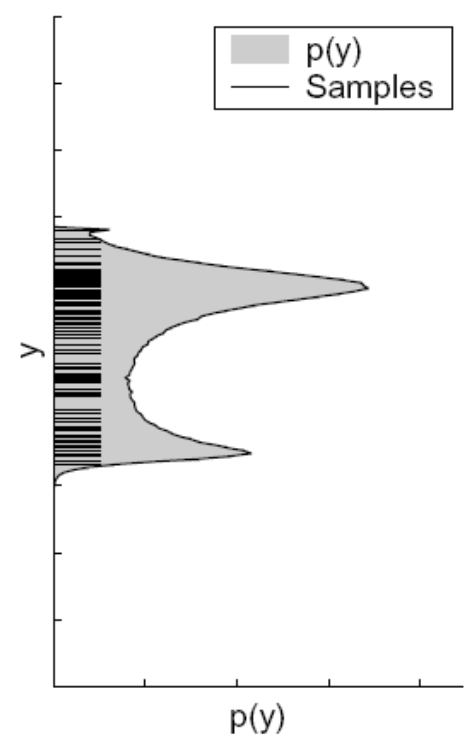
\includegraphics[height=0.45\textwidth]{figures/pf_approx}
	\caption{Approximation of posteriori distribution by samples. Source: \citep{thrun:prob_robo}}
	\label{fig:pf_approx}
\end{figure} 

According to \citet{thrun:prob_robo}, the idea is the posterior's $bel(x_t)$ representation by a random set of samples, drawn from the posteriori. Each sample (resp.\ particle) $x$ at time $t$ is a hypothetical state in state space, resp.\ in true world. The particle set $\chi_t = \left\{ x^{[1]}_t, x^{[2]}_t, \ldots, x^{[m]}_t \right\}$ is the distributions approximation, containing $M$ particles. The \acs{PF}'s algorithm, depicted in figure~\ref{lst:kf}, transforms the $bel(x_{t-1})$, represented by the particle set $\chi_{t-1}$, by incorporating the least control $u_t$ and measurement $z_t$ into the current $bel(x_t)$. Therefor, the algorithm creates first an empty, temporary particle set $\bar{\chi}_t$. Then, the states from $\chi_{t-1}$ are being updated, by incorporating the current control $u_t$. Formally, this done by sampling the new state $x_t$ from the state transition probability $p(x_t|u_t, x^{[m]}_{t-1})$ (line 5). Afterwards, an \emph{importance factor} $w^{[m]}_t$ for the new sample $x^{[m]}_t$ is being calculated (line 6). It is defined as $p(z_t|x^{[m]}_t)$, which is the probability for the measurement $z_t$ given the new state hypothesis, representing a value in true world. The new state hypothesis and its importance factor are stored together, as tuple, in the temporary set $\bar{\chi}_t$ (line 7). The weighted set approximates the $bel(x_t)$.

 Then, the resampling, resp.\ importance sampling, transforms the weighted set, based on their weights into a new set, which represents the new distribution. Therefor, $M$ particles are be drawn according their weight and being inserted in the new set $\chi_t$ (line 14, 15). During this step some particles are being duplicated, usually the ones with high weight, and others, the ones with low weight, are being lost. \citet{thrun:prob_robo} compare it with the Darwinian idea of \emph{survival of the fittest}. According to them, ``it refocuses the particle set to regions in state space with high posteriori probability''.
 
 Instead of the drawing, it is also possible to have a weighted set $\chi_t$, and in every recursion, the weights of the existing particles are being multiplied with their new weight. The method's disadvantage is, that a larger particle set is being required for the same approximation quality, because the particles do not move, they keep their position in state space for every. For this method the particles need to be initialized with weight $1$.
 
\acs{PF}'s can be adaptive, for instance based on the available processing power, the particle set is being increased or decreased \citep{thrun:prob_robo}.

\begin{figure}
\begin{lstlisting}[mathescape]
ParticleFilter($\chi_{t-1}$, $u_t$, $z_t$) {

  $\bar{\chi}_t = \emptyset$
  for $m = 1$ to $M$ {
    sample $x^{[m]}_t \sim p(x_t|u_t, x^{[m]}_{t-1})$
    $w^{[m]}_t = p(z_t|x^{[m]}_t)$
    add $\langle x^{[m]}_t, w^{[m]}_t \rangle$ to $\bar{\chi}_t$
  }
  
  
  \\ resampling
  $\chi_t = \emptyset$
  while size of $\chi_t$ less $M$ {
    draw $i$ with probability $\propto w^{[m]}_t$
    add $x^{[i]}_t$ to $\chi_t$
  }
  
  return $\chi_t$
}
\end{lstlisting}
\caption{Algorithm for \acl{PF} based on \citet{thrun:prob_robo}}
\label{lst:pf}
\end{figure}

\paragraph{Monte Carlo Localization}
\ac{MCL} is a popular localization algorithm often used in the indoor mobile robotics field. The algorithm can deal with a broad range of the before discussed localization problems, especially with the local and global localization problem.

The basic algorithm, shown in figure~\ref{lst:mcl}, is very similar to the \acs{PF} presented in \ref{lst:pf}. Line~5 is being substituted by a method called \texttt{sample\_motion\_model}, which samples the new hypothesis by integrating the control $u_t$ with respect to the robot's motion and its uncertainties during the execution. Furthermore, line~6 is being substituted by the \texttt{measurement\_model}, which depends on the used sensor. It incorporates the sensor's uncertainty to calculate the particle's importance factor. It additionally takes the robot's map into account. Usually it is being used to calculate the importance factor based on the measurement $z_t$, for instance, a distance to a landmark, where the landmark's position is stored in the map. A map can also be used to detect particles at impossible positions to reduce their importance factor. A very detailed description into \acl{MCL} and variations of the algorithm is provided by \citet{thrun:prob_robo}.

A visual example of robot's global localization is shown in figure~\ref{fig:mcl}. The three images show the particles, resp.\ the posteriori $bel(x_k)$ over time. At the beginning the particles are being uniform random particles are spread over the whole state space, because the robot actually does not know where it is, and thus could be positioned anywhere. After moving and gathering sensor data, the particles concentrate in certain regions with higher belief for the robot's position. Thus the posteriori has changed. In the end the particles have concentrated on one spot, hence the robot's confidence of being at this position is very high \citep{thrun:prob_robo}.

\begin{figure}
\begin{lstlisting}[mathescape]
ParticleFilter($\chi_{t-1}$, $u_t$, $z_t$, map) {

  $\bar{\chi}_t = \emptyset$
  for $m = 1$ to $M$ {
    $x^{[m]}_t$ = sample_motion_model($u_t$, $x^{[m]}_{t-1}$)
    $w^{[m]}_t$ = measurement_model($z_t$,$x^{[m]}_t$, map)
    add $\langle x^{[m]}_t, w^{[m]}_t \rangle$ to $\bar{\chi}_t$
  }
  
  
  \\ resampling
  $\chi_t = \emptyset$
  while size of $\chi_t$ less $M$ {
    draw $i$ with probability $\propto w^{[m]}_t$
    add $x^{[i]}_t$ to $\chi_t$
  }
  
  return $\chi_t$
}
\end{lstlisting}
\caption{Basic \acl{MCL} algorithm based on \citet{thrun:prob_robo}}
\label{lst:mcl}
\end{figure}



\begin{figure}[width=0.9\textwidth, height=0.4\textheight]
\subfloat[]{
  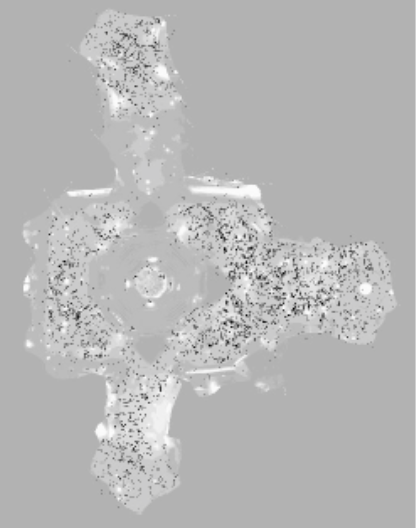
\includegraphics[width=0.3\textwidth]{figures/mcl_1}
}
\subfloat[]{
  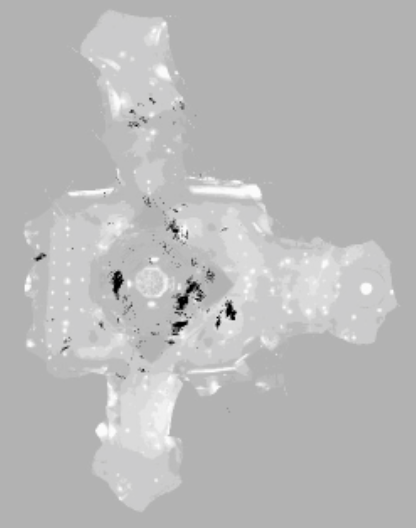
\includegraphics[width=0.3\textwidth]{figures/mcl_2}
}
\subfloat[]{
  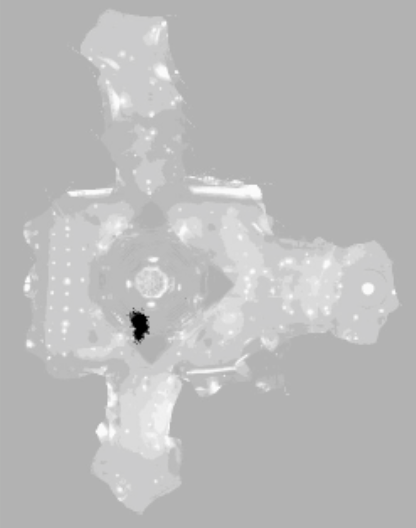
\includegraphics[width=0.3\textwidth]{figures/mcl_3}
}
\caption{Visual example of the \acl{MCL} algorithm. Source:~\citep{thrun:prob_robo}}
\label{fig:mcl}
\end{figure}


\subsubsection*{Related Work}

\citet{Siddiqui:tracking} propose a localization system that uses \acs{PF} and \acs{RSS}-based trilateration of WiFi signals, to track a mobile unit. The approach just relies on sensing \acs{RSS} values, no other sensors are being used. First they collect the \acs{RSS} values in their environment by war-walking. They are being stored together with their location in a lookup table. For their MATLAB simulation they generated a random path with 100 points using the before collected values, which is being tracked during the simulation just based on the \acs{RSS} values. Their simulation simulates a notebook equipped with WiFi, which is being tracked. Thus, their \acs{PF}'s implementation does not sample a new state by integrating the control $u_t$ as shown in (line 5). They used two different weighting functions during their experiment, firstly, a \emph{Gaussian weighting function}, based on the Euclidian distance, and secondly, a \emph{Triangular weighting function} (line 6). According to \citet{Siddiqui:tracking}, they achieved an accurate localization of approx.\ 3~m, as a result of their simulation. During the simulation they assumed, a static environment with sparse activity, and a smooth and continuous motion. They also assumed that no large variations in the signal strength occur over short distances. During their signal recordings they removed the first and last 10\% of the measurements, when the person placed the measuring unit at the position and picked it up again, because they wanted their values to be independent of a human in proximity. Additionally, they neglected outlaws.

\citet{straub:pf} implemented a indoor pedestrian localization and tracking system based on \acs{PF}, which uses a system called \emph{PiNav}, developed at the institute where Straub wrote his thesis, which extracts the person's motion in form of step frequency, step size, and heading. Therefor, the person need to be equipped with the hip-mounted PiNav-System, which includes a accelerometer, gyroscope and a compass. Additionally, his solution uses an accessibility map, which is based on a Neural Network, to learn which space on a map is accessible by pedestrians. By fusing the pedestrian's motion and the accessibility map in a \acs{PF}, his solution achieves an average accuracy of 1.1~m \citep{straub:pf}.

\citet{wang:wlan} proposes a \acs{RSS} based WiFi positioning system using particle filter to fuse the location estimated via WiFi with additional map and accelerometer data. Their system uses the above mentioned scene analysis, especially the k-Nearest Neighbors algorithm for the positioning. During the offline stage fingerprints of the WiFi signal are being collected in one meter distance to the access points. During the localization, resp.\ the online stage, the algorithm compares the fingerprints of the collected WiFi signals with the stored ones from the offline stage and returns a location estimation. According to \citet{wang:wlan}, the 3-axis accelerometer's values can be used in theory to estimate the traveled distance by integrating the values. But, due to the low signals and the sensor's noise it does not work in praxis. Thus, the use a zero-crossing approach to detect steps and estimate their size. The zero-crossing approach just detects if the vertical acceleration crosses the zero-line. Additionally, their solution uses the environments map to sort out impossible particles, like particles crossing a wall.
Their simulation results show, that by using map and accelerometer in addition to kNN, improves the location error by 40\%. Their solution is also 30\% better than the \ac{KF}'s result. During their real world tests, they achieved a mean error of 4.3~m with a standard deviation of 2.8~m \citep{wang:wlan}.

\citep{siddiqi:experiments_mcl_wifi} uses \acs{MCL} to globally localize a \emph{Pioneer 2DX} robot in an indoor environment using the robots odometers and the measured \acs{RSS} of WiFi signals. The algorithm's action model is based on the data which is measured by the odometers, which deliver data for short distances with a very good accuracy. The motion is being split up into translations and rotations. The action model, resp.\ motion model, samples the motion with different uncertainties for translation and rotation. The observation model, resp.\ measurement model, uses a signal strength map, which is split up into a grid with squared fields with 0.5~m size. Before localization can take place, for each grid cell the \acs{RSS} of each WiFi access point needs to be measured to store \acs{RSS} mean and standard deviation. Due to the fact, that \citet{siddiqi:experiments_mcl_wifi} assumes that the signal attenuation does not change on short distances, they just measured it for a few fields and assumed the same value for the neighbor fields. During the localization the actual \acs{RSS} values are being compared with the collected one for the importance factor. The observation model also weeds out particles, by using the map constraints, which already without \acs{RSS} comparison enables very good localization \citep{siddiqi:experiments_mcl_wifi}. The robot's orientation $\theta$ is not taken into account by the observation model.
During their tests they found out, that by increasing the amount of access points, the location error decreases \citep{siddiqi:experiments_mcl_wifi}. They also mention that their approach should also work for localization of humans instead of robots, but a robot's motion model is simpler than the one of a human. According to \citet{siddiqi:experiments_mcl_wifi}, they achieved during most test cases a accurate localization with approx.\ 2~m error.
% global localization robot with wifi, signal strength map
% odometrie action model
% observation model based on signal s map Pioneer 2DX robot
% show empirically that with more aps higher accuracy
% easier with robot than with person
% rotation and translation in small steps with different gaussian noise, very good odometry
% added more noise than required

%observatoin model: map constraints, weed out particles that are not on map. This enables good localization without use of signal strength
% envirionment was split in grid of 0.5 m squares, for each grid signalstrength was measured , mean and variance for each ap in grid
% \theta is not taken into account in observation model.